%%%
%
% $Autor: Wings $
% $Datum: 2021-05-14 $
% $Pfad: GitLab/CornerBlending $
% $Dateiname: ArcStrategy
% $Version: 4620 $
%
% !TeX spellcheck = de_GB
%
%%%






\chapter{Verrundung mit einem Kreisbogen}

%todo Siehe \cite{Walton:2009} p.88, chapter 2.1.

\section{Gleichungen}

Blending with an arc is a simple variant of smoothing corners. This variant enables the processing and the generation of files according to DIN 66025. For smoothing, three points $P_0$ and $S$ and $P_1$ are always considered, thus a symmetric Hermite problem results. According to theorem \ref{StrategySymmetricDefStandardHP} it is assumed to be in the standard form $HP(L,\alpha)$.
 
 \bigskip
 
 
 
 \begin{figure}[h]
 %\centering
 %\includegraphics[width=.9\textwidth]{Sin2/Eckenglaettung11}
 
 
 \begin{center}
   \begin{tikzpicture}[scale=2]
 
     \coordinate[label=left:$P_0$]  (P0) at (2,0);
     \coordinate[label=right:$S$] 
        (PS) at (4,0);
     \coordinate[label=left:$P_1$] (P1) at (3.0,1.75);
     \coordinate[label=left:$M$] (M) at (2.0,1.2);
     
     \coordinate%[label=left:$P_i$]
       (P01) at
     ({4*(1.-0.5)+2.309265589*0.5*cos(-30)}, {2.309265589*0.5+2.309265589*0.5*sin(-30)});
     
     \coordinate[label=left:$\frac{\alpha}{2}$] (alpha) at (3.7,0.1);
 
     \coordinate[label=below:$L$](c) at ($ (P0)!.5!(PS) $);
     \coordinate[label=above:$r$] (b) at ($ (PS)!.75!(M) $);
     \coordinate[label=above:$+$] (b1) at ($ (PS)!.5!(M) $);
     \coordinate[label=above:$\varepsilon$] (b2) at ($ (PS)!.25!(M) $);
     \coordinate[label=left:$r$](a) at ($ (P0)!.5!(M) $);
 
     % draw the background
     \draw [line width=1.0pt] (P0) -- (PS);
     \draw [line width=1.0pt] (PS) --(P1);
     \draw [dotted,line width=1.0pt,blue] (PS) --(P01);
     \draw [line width=1.0pt,blue] (P01) --(M);
     \draw [line width=1.0pt,blue] (P0) --(M);
 %    \node[draw,circle through={(M)}] (Zentrum) {};
 
 
    \draw [red,line width=1.5pt,domain=-90:30] plot ({4*(1.-0.5)+2.309265589*0.5*cos(\x)}, {2.309265589*0.5+2.309265589*0.5*sin(\x)});
 
    \draw [green,line width=0.5pt,domain=180:150] plot ({4*(1.)+0.75*cos(\x)}, {0.75*sin(\x)});
 
     \node (P0) at (P0) {$\bullet$};
     \node (PS) at (PS) {$\bullet$};
     \node (M) at (M) {$\bullet$};
     \node (P1) at (P1) {$\bullet$};
 
   \end{tikzpicture}
 \end{center}
 \caption{Smoothing a corner with the help of an arc - triangle}\label{KreisglaettungDreieck}
 \end{figure}
 
 
 The figure \ref{CircleGlazingTriangle} represents the situation.  The points $P_0$, $S$ and $P_1$ are given. The included angle $\alpha = \angle(P_0;S;P_1)$ as well as the distance $L=\|\|S-P_0\|\| =\|\|P_1-S\|\|$ are shown in the graph.  The red arc is the desired result. The distance of its centre $M$ to $S$ is then $r+\varepsilon$, where $r$ is the radius of the arc and $\varepsilon$ is the given tolerance. Thus we obtain a right triangle $P_0SM$ whose edge lengths are $L$, $r+\varepsilon$ and $r$.

\bigskip

According to the definition of the sine and the tangent, it follows:
 
 $$\sin\left(\frac{\alpha}{2}\right)= \frac{L}{r+\varepsilon}
 \qquad \hbox{und}\qquad \tan\left(\frac{\alpha}{2}\right)= \frac{L}{r}$$
 
 $$\Leftrightarrow\quad 
 \varepsilon = \frac{L}{\sin\left(\frac{\alpha}{2}\right)} - r
 \qquad \hbox{und}\qquad 
  r = \cot\left(\frac{\alpha}{2}\right) L$$
 
 The two equations can be combined to give the following conditions:
 
 $$\varepsilon = L \cdot \frac{1-\cos\left(\frac{\alpha}{2}\right)}{\sin\left(\frac{\alpha}{2}\right)}
 \qquad \hbox{bzw.} \qquad  L = \varepsilon \cdot \frac{\sin\left(\frac{\alpha}{2}\right)}{1-\cos\left(\frac{\alpha}{2}\right)}$$
 
 This gives the equation for the radius:
 
 $$r = L \cdot \cot\left(\frac{\alpha}{2}\right)
 = L \cdot \sqrt{\frac{1-\cos(\alpha)}{1+\cos(\alpha}}
 = L \cdot \frac{\sin(\alpha)}{1+\cos(\alpha)} = L \cdot \frac{P_{1,x}}{P_{1,y}}$$
 
 
 The factor for converting $L$ and $\varepsilon$ can be simplified using trigonometric transformations.
 
 
 \bigskip
 
 
 $$\frac{1-\cos\left(\frac{\alpha}{2}\right)}{\sin\left(\frac{\alpha}{2}\right)}
 =
 \frac{1-\sqrt{\frac{1-\cos(\alpha)}{2}}}{\sqrt{\frac{1+\cos(\alpha)}{2}}}
 =
  \frac{\sqrt{2}-\sqrt{1-\cos(\alpha)}}{\sqrt{1+\cos(\alpha)}}
 = 
 \frac{\sqrt{1+\cos(\alpha)}-\sin(\alpha) }{1+\cos(\alpha)}
 $$
 
 By comparing this with the symmetric Hermite problem in standard form, the following notation is then obtained:
 
  
 $$\frac{1-\cos\left(\frac{\alpha}{2}\right)}{\sin\left(\frac{\alpha}{2}\right)}
 =
 \frac{\sqrt{P_{1,x}}-P_{1,y}}{P_{1,x}}
 $$
 
 The previous considerations are now summarised in the following sentence.
 
 \bigskip
 
 \SATZ{\label{KreisstrategieKreis}
  Let a symmetric Hermite problem $(P_0,\, \vec{t}_0,\,P_1,\, \vec{t}_1,S,L)$ be given. Without restriction of generality, it is in the standard form

  $$
    \left\{\binom{0}{0},\, \binom{1}{0},\,
      \binom{L+L\cdot \cos(\alpha)}{L\cdot \sin(\alpha)},\, \binom{\cos(\alpha)}{\sin(\alpha)},\, \binom{L}{0},L
    \right\}
  $$

  with $L\in \R^{>0}$ uad $\alpha \in (-\pi;\, \pi] $.
  
  \medskip
  
  
  Then an arc can be found that connects the points $P_0$ and $P_1$, has the same tangent directions at the two points.
  
  \medskip
  
  For the circular arcs applies:
  
  $$
    r
    = 
    L \cdot \left| \frac{P_{1,x}}{P_{1,y}}\right|; \quad 
    \phi_0 = -\sign(\alpha)  \cdot \frac{\pi}{2}; \quad
    \phi_1-\phi_0 
    = 
    \sign(\alpha)  \cdot \pi - \alpha = \beta; 
  $$
        
  $$
    M 
    = P_0 + \sign(\alpha) \cdot r \cdot \vec{t}_0^\perp 
    =       \sign(\alpha) \cdot r \cdot \binom{0}{1}
  $$
 }
 
 \bigskip
 
From the specification of the distance $L$, the maximum error can be calculated, as shown in theorem \ref{CircleStrategyCircle}. According to the derivation, it is also possible to specify the maximum error $\varepsilon$ and determine the maximum distance $L$ from it.
 
 
\bigskip
 
\SATZ{\label{KreisstrategieLEps} 
   Let a symmetric Hermite problem $(P_0,\, \vec{t}_0,\,P_1,\, \vec{t}_1,S,L)$ be given. Without restriction of generality, it is in the standard form
  
   $$\left\{\binom{0}{0},\, \binom{1}{0},\,
  \binom{L+L\cdot \cos(\alpha)}{L\cdot \sin(\alpha)},\, \binom{\cos(\alpha)}{\sin(\alpha)},\, \binom{L}{0},L\right\}$$
  
  with $L\in \R^{>0}$ and $\alpha \in (-\pi;\, \pi] $.
   
  \medskip
   
  \begin{itemize}
    \item [a)] Let the maximum error $\varepsilon$ be given. The maximum distance $L$ for which an arc exists according to the theorem \ref{CircleStrategyCircle} that takes the error into account is given by:
         
         $$L(\varepsilon,\alpha) 
           =
           \varepsilon \cdot \frac{P_{1,x}}{\sqrt{P_{1,x}}-P_{1,y}}
           =
           \varepsilon \cdot \frac{L+L\cdot \cos(\alpha)}{\sqrt{L+L\cdot \cos(\alpha)}-L+L\cdot \cos(\alpha)}
         $$
          
    \item [b)] When the distance $L$ is specified, the following maximum error results:         
         
          $$
            \varepsilon(L,\alpha) 
            = 
            L \cdot  \frac{\sqrt{P_{1,x}}-P_{1,y}}{P_{1,x}}
            =
            L \cdot \frac{\sqrt{L+L\cdot \cos(\alpha)}-L+L\cdot \cos(\alpha)}{L+L\cdot \cos(\alpha)}
           $$
   \end{itemize}
} 
 
 
%\section{Kreis}
%\subsection{Darstellung eines Punktes auf einem Kreis}
%Darstellung eines beliebigen Punktes auf einer Kurve in Abhängigkeit eines Parameters $\lambda$. \linebreak
%
%\begin{equation}
%\vec{p}(\lambda)=\binom{p_x(\lambda)}{p_y(\lambda)}
%\end{equation}
%
%
%Befindet sich der Punkt auf einem Kreis mit dem Radius r und dem Mittelpunkt $\vec{m}=\binom{m_x}{m_y}$ des Kreises auch der Ursprung des Koordinatensystem, so kann man jeden beliebigen Punkt auf dem Kreis in Abhängigkeit des Winkles $\alpha \in [0;2\pi]$  darstellen.\linebreak
%Die Funktion C($\alpha$) entspricht dann:
%
%\begin{equation}
%C(\alpha)=\vec{m}+r*\binom{p_x(\alpha)}{p_y(\alpha)}
%\end{equation}
%
%
%Der Punkt lässt sich in X und Y-Komponenten aufteilen
%
%\subsection{Implizite Kreisdarstellung}
%Mit Hilfe von Phytagoras ergibt sich die implizite Kreisdarstellung :
%
%\begin{equation}
%(p_x-m_x)^2+(p_y-m_y)^2=r^2
%\end{equation}
%
%Daraus ergibt sich für die Strecke vom Ursprung zu $p_x$ bzw. $p_y$:
%
%\begin{eqnarray}
%p_x=&m_x+r\cdot\cos(\alpha)\\
%p_y=&m_y+r\cdot\sin(\alpha)
%\end{eqnarray}
%
%
%
%
%\subsection{Explizite Kreisdarstellung}
%Eine Funktion für die für die explizite Darstellung eines Punktes auf einem Kreis lautet dann:
%
%\begin{equation}
%C(\alpha)=\vec{m}+r\cdot\binom{\cos(\alpha)}{\sin(\alpha)}
%\end{equation}
%Siehe hierzu auch Kapitel 5. Kreis 
%
%%\subsection{Kreisbogen}
%
%\begin{equation}
%B: \begin{cases}
%[\varphi_0; \varphi_0 + \alpha] &\rightarrow \mathbb{R}^2 \\
%\varphi&\mapsto\vec{m}+r\cdot\binom{\cos(\varphi)}{\sin(\varphi)}
%\end{cases}
%\end{equation}




%todo Quelle

\bigskip

These considerations result in limitations for the use of this strategy, which are summarised in the following comment.


\bigskip



\Bemerkung
{
  The following conditions for applying the strategy of a circle must be fulfilled:

  \begin{itemize}
    \item [a)] $$P_0 \neq P_1$$
    \item [b)] $$ \vec{t}_0 = -\vec{t}_1\quad \Leftrightarrow \quad \alpha = 0$$
    \item [c)] $$ \vec{t}_0 =  \vec{t}_1\quad \Leftrightarrow \quad \alpha = \pi$$
  \end{itemize}
}


\section{Bewertung}

Rounding by means of a circular arc leads to a continuous course of the angle change. The figure \ref{circlestrategyangle} illustrates this.

\bigskip

\begin{figure}
  \begin{center}
    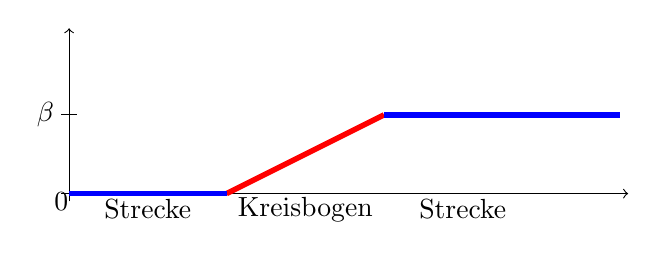
\begin{tikzpicture}
       \draw [->] (0,-0.1) -- (0,2.1);
       \draw [->] (-0.1,0) -- (7.1,0);
       \draw (-0.1,1) -- (0.1,1);
       
       \node (R) at (-0.3,1) {$\beta$};
       \node (O) at(-0.1,-0.1) {$0$};
       
       
       \node (P0) at (1,-0.2) {Strecke};
       \node (P0) at (3,-0.2) {Kreisbogen};
       \node (P0) at (5,-0.2) {Strecke};
       \draw [line width=2pt,color=red] (2,0) -- (4,1);
       \draw [line width=2pt,color=blue] (0,0) -- (2,0);
       \draw [line width=2pt,color=blue] (4,1) -- (7,1);
       
    \end{tikzpicture}
  \end{center}
  \caption{Angular change with blending arc}\label{KreisstrategieWinkel}
\end{figure}

\bigskip

Due to the rounding with a circular arc, the curvature of the curve is not continuous. The figure \ref{CircleStrategyCurvature} shows that the curvature is constant in the range of distances $0$ and on the circular arc with the value $\frac{1}{r}$, where $r$ is the radius of the circular arc used. Due to the formula $a=\frac{v^2}{r}$ for a movement on a circular arc, the acceleration course exhibits continuity jumps at the transitions for a constant path velocity.


\begin{figure}
  \begin{center}
    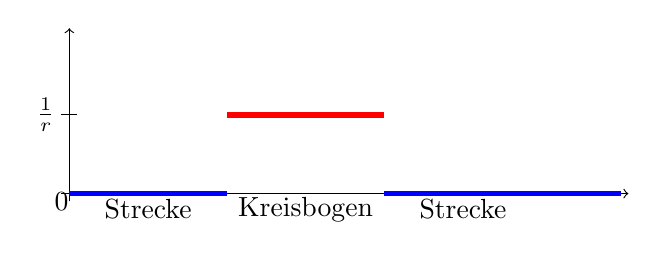
\begin{tikzpicture}
       \draw [->] (0,-0.1) -- (0,2.1);
       \draw [->] (-0.1,0) -- (7.1,0);
       \draw (-0.1,1) -- (0.1,1);
       
       \node (R) at (-0.3,1) {$\frac{1}{r}$};
       \node (O) at(-0.1,-0.1) {$0$};
       
       
       \node (P0) at (1,-0.2) {Strecke};
       \node (P0) at (3,-0.2) {Kreisbogen};
       \node (P0) at (5,-0.2) {Strecke};
       \draw [line width=2pt,color=red] (2,1) -- (4,1);
       \draw [line width=2pt,color=blue] (0,0) -- (2,0);
       \draw [line width=2pt,color=blue] (4,0) -- (7,0);
       
    \end{tikzpicture}
  \end{center}
  \caption{Curvature progression  for a blending arc}\label{KreisstrategieKruemmung}
\end{figure}

\bigskip

Depending on the angle change $\beta$ at the corner $S$ and the tolerance $\varepsilon$, the maximum length of the shortening of the lines can be calculated. The figure~\ref{Circle strategyL} shows the corresponding diagram, where the tolerance $\varepsilon$ is set to the value $1$.
 
 
\begin{figure}
  \begin{center}
    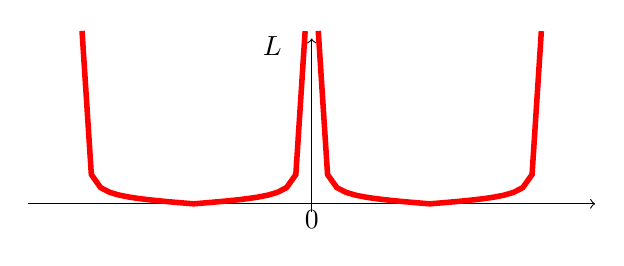
\begin{tikzpicture}[declare function ={Leps(\a) =sqrt(abs(sin(180-\a)*(sin(180-\a)-1)))/abs(10*sin(180-\a)-1);}]
    \draw [->] (3.5,-0.1) -- (3.5,2.1);
    \draw [->] (-0.1,0) -- (7.1,0);
    
    \node (R) at (3.0,2) {$L$};
    \node (O) at(3.5,-0.2) {$0$};
    
    \draw [red,line width=2pt,domain=175:5] plot({3.5-\x/60},{Leps(\x)});
    \draw [red,line width=2pt,domain=5:175] plot({3.5+\x/60},{Leps(\x)});
  
    
    
    \end{tikzpicture}
  \end{center}
  \caption{Maximum range for a blending arc of a circle - $L(\varepsilon=const, \alpha)$}\label{KreisstrategieL}
\end{figure}


\bigskip

The area provided can also be specified. Depending on the distance $L$ from the corner point $S$, the deviation $\varepsilon$ can be calculated. The figure \ref{Circle StrategyEps} represents the function as a function of $L$ and the angle $\alpha$.



 
\begin{figure}
  \begin{center}
    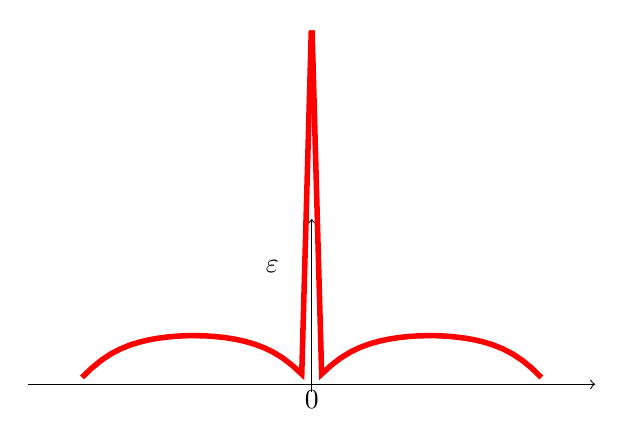
\begin{tikzpicture}[declare function ={EpsL(\x) =sqrt(1+1/(4*sin(180-\x)*sin(180-\x)))-1/(2*sin(180-\x));
    }]
    \draw [->] (3.5,-0.1) -- (3.5,2.1);
    \draw [->] (-0.1,0) -- (7.1,0);
    
    \node (R) at (3,1.5) {$\varepsilon$};
    \node (O) at(3.5,-0.2) {$0$};
    
   \draw [red,line width=2pt,domain=0.3:175] plot({3.5-\x/60},{EpsL(\x)/1});
   \draw [red,line width=2pt,domain=0.3:175] plot({3.5+\x/60},{EpsL(\x)/1});
    
    
    
    \end{tikzpicture}
  \end{center}
  \caption{Deviation when specifying the distance $L$ when rounding with a circular arc}\label{KreisstrategieEps}
\end{figure}


The figures \ref{Circle StrategyL} and \ref{Circle StrategyEps} show the curves of the length as a function of the angle change for a fixed tolerance and the error as a function of the angle change for a given length. If the angle change is minimal, then the error or length $L$ is extreme. In this case, rounding by means of an arc is not possible. In order to develop a sensible strategy, a minimum angle change must be specified from which a blemnding arc is permitted. Likewise, a maximum angle change must also be defined. For an angular change of $\pm \pi$ is a bend. In this case, a blending is also not possible.




\section{Examples}

\BEISPIEL
{
  Let it be the symmetric Hermite problem 

  $$\left\{\binom{0}{0},\, \binom{1}{0},\,
    \binom{6.0+6.0\cdot \cos\left(\frac{2}{3}\pi\right)}{6.0\cdot \sin\left(\frac{2}{3}\pi\right)},\, \binom{\cos\left(\frac{2}{3}\pi\right)}{\sin\left(\frac{2}{3}\pi\right)},\, \binom{6.0}{0},6.0\right\}
  $$

  with $L=6$ and $\alpha=\frac{2}{3}\pi$.

  For the blending arc follows:

  $$M=\binom{0}{3,4641}; \quad r=3,46412;\quad \phi_0 = -\frac{\pi}{2}; \quad \alpha=\frac{2}{3}\pi$$

  \begin{center}
    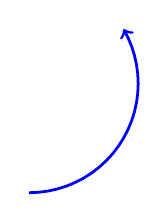
\begin{tikzpicture}[scale=0.4]
      \begin{scope}
        \HermiteSym{1}{120}
      \end{scope}

      \begin{scope}[shift={(12cm,0cm)}]
        \HermiteSym{1}{120}
        \draw [blue,line width=1pt,domain=-90:30,->] plot ({0+3.464101612*cos(\x)}, {3.464101612+3.464101612*sin(\x)});
      \end{scope}
    \end{tikzpicture}
  \end{center}
}


\BEISPIEL
{
  Let it be the symmetric Hermite problem 
  
  $$\left\{\binom{0}{0},\, \binom{1}{0},\,
  \binom{6.0+6.0\cdot \cos\left(\frac{7}{18}\pi\right)}{6.0\cdot \sin\left(\frac{7}{18}\pi\right)},\, \binom{\cos\left(\frac{7}{18}\pi\right)}{\sin\left(\frac{7}{18}\pi\right)},\, \binom{6.0}{0},6.0\right\}$$
  
  with $L=6$ and $\alpha=\frac{7}{18}\pi$.
  
  For the blending arc follows:
  
  $$M=\binom{0}{8,5689}; \quad r=8,5689;\quad \phi_0 = -\frac{\pi}{2}; \quad \alpha=\frac{7}{18}\pi$$
  
  
  \begin{center}
    \begin{tikzpicture}[scale=0.4]
    \begin{scope}
    \HermiteSym{1}{70}
    \end{scope}
    
    \begin{scope}[shift={(12cm,0cm)}]
    \HermiteSym{1}{70}
    \draw [blue,line width=1pt,domain=-90:-20,->] plot ({0+8.568888035*cos(\x)}, {8.568888035+8.568888035*sin(\x)});
    \end{scope}
    \end{tikzpicture}
  \end{center}
}



\BEISPIEL
{
  Let it be the symmetric Hermite problem 
  
  $$\left\{\binom{0}{0},\, \binom{1}{0},\,
  \binom{6.0+6.0\cdot \cos\left(\frac{1}{9}\pi\right)}{6.0\cdot \sin\left(\frac{1}{9}\pi\right)},\, \binom{\cos\left(\frac{1}{9}\pi\right)}{\sin\left(\frac{1}{9}\pi\right)},\, \binom{6.0}{0},6.0\right\}$$
  
  with $L=6$ and $\alpha=\frac{1}{9}\pi$.
  
  For the blending arc follows:
  
  $$M=\binom{0}{34,0277}; \quad r=34,0277;\quad \phi_0 = -\frac{\pi}{2}; \quad \alpha=\frac{1}{9}\pi$$
  
  
  \begin{center}
    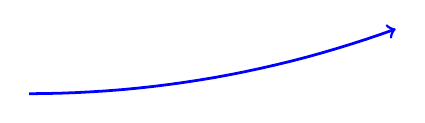
\begin{tikzpicture}[scale=0.4]
    \begin{scope}
    \HermiteSym{1}{20}
    \end{scope}
    
    \begin{scope}[shift={(12cm,0cm)}]
    \HermiteSym{1}{20}
    \draw [blue,line width=1pt,domain=-90:-70,->] plot ({0+34.02769092*cos(\x)}, {34.02769092+34.02769092*sin(\x)});
    \end{scope}
    \end{tikzpicture}
  \end{center}
}


\BEISPIEL
{
  Let it be the symmetric Hermite problem 
  
  $$\left\{\binom{0}{0},\, \binom{1}{0},\,
  \binom{12.0}{0},\, \binom{1}{0},\, \binom{6.0}{0},6.0\right\}$$
  
  with $L=6$ and $\alpha=0$.
  
 There is no blending arc here.

  
  \begin{center}
    \begin{tikzpicture}[scale=0.4]
    \begin{scope}
    \HermiteSym{1}{0}
    \end{scope}
    
    \end{tikzpicture}
  \end{center}
}



\BEISPIEL
{
  Let it be the symmetric Hermite problem 
  
  $$\left\{\binom{0}{0},\, \binom{1}{0},\,
  \binom{6.0+6.0\cdot \cos\left(-\frac{1}{9}\pi\right)}{6.0\cdot \sin\left(-\frac{1}{9}\pi\right)},\, \binom{\cos\left(-\frac{1}{9}\pi\right)}{\sin\left(-\frac{1}{9}\pi\right)},\, \binom{6.0}{0},6.0\right\}$$
  
  with $L=6$ and $\alpha=-\frac{1}{9}\pi$.
  
  For the blending arc follows:
  
  $$M=\binom{0}{-34,0277}; \quad r=34,0277;\quad \phi_0 = \frac{\pi}{2}; \quad \alpha=\frac{1}{9}\pi$$
  
  
  \begin{center}
    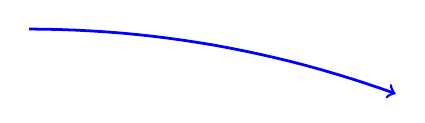
\begin{tikzpicture}[scale=0.4]
    \begin{scope}
    \HermiteSymNeg{1}{-20}
    \end{scope}
    
    \begin{scope}[shift={(12cm,0cm)}]
    \HermiteSymNeg{1}{-20}
    \draw [blue,line width=1pt,domain=90:70,->] plot ({0+34.02769092*cos(\x)}, {-34.02769092+34.02769092*sin(\x)});
    \end{scope}
    \end{tikzpicture}
  \end{center}
}



\BEISPIEL
{
  Let it be the symmetric Hermite problem 
  
  $$\left\{\binom{0}{0},\, \binom{1}{0},\,
  \binom{6.0+6.0\cdot \cos\left(-\frac{7}{18}\pi\right)}{6.0\cdot \sin\left(-\frac{7}{18}\pi\right)},\, \binom{\cos\left(-\frac{7}{18}\pi\right)}{\sin\left(-\frac{7}{18}\pi\right)},\, \binom{6.0}{0},6.0\right\}$$
  
  with $L=6$ and $\alpha=-\frac{7}{18}\pi$.
  
  For the blending arc follows:
  
  $$M=\binom{0}{-8,5689}; \quad r=8,5689;\quad \phi_0 = \frac{\pi}{2}; \quad \alpha=-\frac{7}{18}\pi$$
  
  
  \begin{center}
    \begin{tikzpicture}[scale=0.4]
    \begin{scope}
    \HermiteSymNeg{1}{-70}
    \end{scope}
    
    \begin{scope}[shift={(12cm,0cm)}]
    \HermiteSymNeg{1}{-70}
    \draw [blue,line width=1pt,domain=90:20,->] plot ({0+8.568888035*cos(\x)}, {-8.568888035+8.568888035*sin(\x)});
    \end{scope}
    \end{tikzpicture}
  \end{center}
}


\BEISPIEL
{
  Let it be the symmetric Hermite problem 
  
  $$\left\{\binom{0}{0},\, \binom{1}{0},\,
  \binom{6.0+6.0\cdot \cos\left(-\frac{2}{3}\pi\right)}{6.0\cdot \sin\left(-\frac{2}{3}\pi\right)},\, \binom{\cos\left(-\frac{2}{3}\pi\right)}{\sin\left(-\frac{2}{3}\pi\right)},\, \binom{6.0}{0},6.0\right\}$$
  
  with $L=6$ and $\alpha=-\frac{2}{3}\pi$.
  
  For the blending arc follows:
  
  
  $$M=\binom{0}{-3,4641}; \quad r=3,46412;\quad \phi_0 = \frac{\pi}{2}; \quad \alpha=-\frac{2}{3}\pi$$
  
  
  \begin{center}
    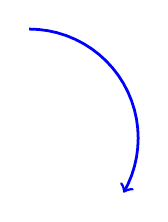
\begin{tikzpicture}[scale=0.4]
    \begin{scope}
    \HermiteSymNeg{1}{-120}
    \end{scope}
    
    \begin{scope}[shift={(12cm,0cm)}]
    \HermiteSymNeg{1}{-120}
    \draw [blue,line width=1pt,domain=90:-30,->] plot ({0+3.464101612*cos(\x)}, {-3.464101612+3.464101612*sin(\x)});
    \end{scope}
    \end{tikzpicture}
  \end{center}  
}



%todo Weiterführende Themen
%\section{Todo}
%\textcolor{red}{Kreis-Kreis-Übergang}
%\textcolor{red}{Gerade-Kreis-Übergang}
